% 48-19(48쪽) — $x$축 위의 점 A 에서 만나는 $y=\log_a x$, $y=\log_{\frac13}x$ 와 직선 $x=9$ 가 만드는 삼각형 ABC(원문 「오른쪽 그림」). 스캔 화질이 낮아 TikZ 로 다시 그림.
% 라벨은 원문에 있는 것만 — 두 곡선 이름, 점 A·B·C, 직선 $x=9$ 와 눈금 9, 원점 O. 밑 $a$(답)는 그림에서 읽히지 않게 적지 않는다.
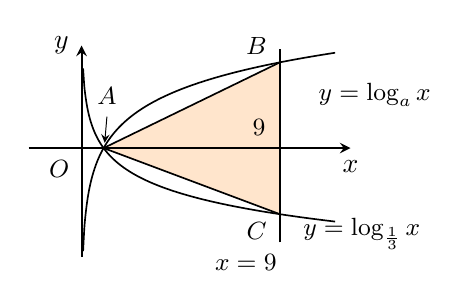
\begin{tikzpicture}[line width=0.6pt, x=0.28cm, y=0.42cm, >=stealth]
  \fill[orange!20] (1,0) -- (9,2.593) -- (9,-2.0) -- cycle;
  \draw[->, line width=0.7pt] (-2.4,0) -- (12.2,0) node[below=1pt] {$x$};
  \draw[->, line width=0.7pt] (0,-3.3) -- (0,3.1) node[left=1pt] {$y$};
  \draw[line width=0.7pt] (9,-2.85) -- (9,3.0);
  \draw[domain=0.07:11.5, samples=200, smooth] plot (\x, {1.18*ln(\x)});
  \draw[domain=0.07:11.5, samples=200, smooth] plot (\x, {-ln(\x)/ln(3)});
  \draw (1,0) -- (9,2.593) (1,0) -- (9,-2.0);
  \draw[->, line width=0.35pt] (1.15,0.95) -- (1.05,0.16);
  \node[font=\small, anchor=south] at (1.15,1.02) {$\pt{A}$};
  \node[font=\small, anchor=south east] at (8.85,2.52) {$\pt{B}$};
  \node[font=\small, anchor=north east] at (8.85,-1.95) {$\pt{C}$};
  \node[font=\small, anchor=south east] at (8.80,0.08) {$9$};
  \node[font=\small, anchor=north east] at (9.3,-2.92) {$x=9$};
  \node[font=\small, anchor=west] at (10.3,1.60) {$y=\log_a x$};
  \node[font=\small, anchor=west] at (9.6,-2.60) {$y=\log_{\frac{1}{3}} x$};
  \node[font=\small, anchor=north east] at (-0.10,-0.06) {$\pt{O}$};
\end{tikzpicture}
